\documentclass[12pt]{beamer}

\usepackage{beamerthemeCambridgeUS}
\usepackage{textpos}
\usepackage{ragged2e}

\graphicspath{{G:/My Drive/FIGURAS/}}

\title[Introducción]{GEOMORFOLOGÍA}
\author[Edier Aristizábal]{Edier V. Aristizábal G.}
\institute{\emph{evaristizabalg@unal.edu.co}}
\date{Version:\today}

\addtobeamertemplate{headline}{}{%
	\begin{textblock*}{2mm}(.9\textwidth,0cm)
	\hfill\includegraphics[height=1cm]{un}  
	\end{textblock*}}

\begin{document}
%%%%%%%%%%%%%%%%%%%%%%%%%%%%%%%%%%%%%%%%%%%%%%%%%%%%%%%%%%%%%%%%
\begin{frame}
\titlepage
\centering
\includegraphics[width=5cm]{unal}\hspace*{4.75cm}~%
\includegraphics[width=2cm]{logo3} 
\end{frame}
%%%%%%%%%%%%%%%%%%%%%%%%%%%%%%%%%%%%%%%%%%%%%%%%%%%%%%%%%%%%%%%%
\begin{frame}
\frametitle{Motivación}
\framesubtitle{\textbf{Geomorfología}: Ciencia que estudia la forma de la superficie de la Tierra y los procesos que las originan}
\emph{Geo} = \textbf{Tierra}; \emph{morphos} = \textbf{forma}; \emph{logy} = \textbf{ciencia}
\centering
\includegraphics[width=8cm]{geo}
\end{frame}
%%%%%%%%%%%%%%%%%%%%%%%%%%%%%%%%%%%%%%%%%%%%%%%%%%%%%%%%%%%%%%%%%
\begin{frame}
\frametitle{Motivación}
\framesubtitle{Por qué estudiar la geomorfología?}
Entender el paisaje es clave para:
\begin{columns}
		\begin{column}{.3\linewidth}
\begin{itemize}
\small{
\item Entender los hábitat de los organismos (incluyendo los humanos)
\item Ordenar el territorio
\item Evaluar las amenazas
\item Evaluar los impactos ambientales
\item Intervenir el territorio adecuadamente
\item La geomorfología nos provee de una nueva forma del ver el paisaje…}
\end{itemize}
		\end{column}
		\begin{column}{.7\linewidth}
		\begin{center}
		\includegraphics[width=10cm]{earth2}
		\end{center}
		\end{column}
	\end{columns}
\end{frame}
%%%%%%%%%%%%%%%%%%%%%%%%%%%%%%%%%%%%%%%%%%%%%%%%%%%%%%%%%%%%%%%%%%
\begin{frame}
\frametitle{Motivación}
\small{\emph{La mayor parte de la superficie terrestre es agua, y la mayor parte de la superficie terrestre continental es menor a $2$ km de altura}}
\begin{center}
\includegraphics[width=11cm]{area}
\end{center}
\end{frame}
%%%%%%%%%%%%%%%%%%%%%%%%%%%%%%%%%%%%%%%%%%%%%%%%%%%%%%%%%%%%%%%%%%
\begin{frame}
\begin{center}
\small{\emph{Pero la mejor razón de todas para estudiar geomorfología es por que el paisaje es simplemente fascinante e increíblemente bello}}
\includegraphics[width=9cm]{imagen}
\end{center}
\end{frame}
%%%%%%%%%%%%%%%%%%%%%%%%%%%%%%%%%%%%%%%%%%%%%%%%%%%%%%%%%%%%%%%%%%
\begin{frame}
\frametitle{Curso: Geomorfología}
\justifying
\small{
La información del curso, tales como programa, lecturas recomendadas y demás podrá ser consultado en Classroom:\vfill
\begin{center}
\url{https://classroom.google.com/u/0/c/NjI0Mjg5NTg3NTda}\\
Class code: [zap5jhd]\\
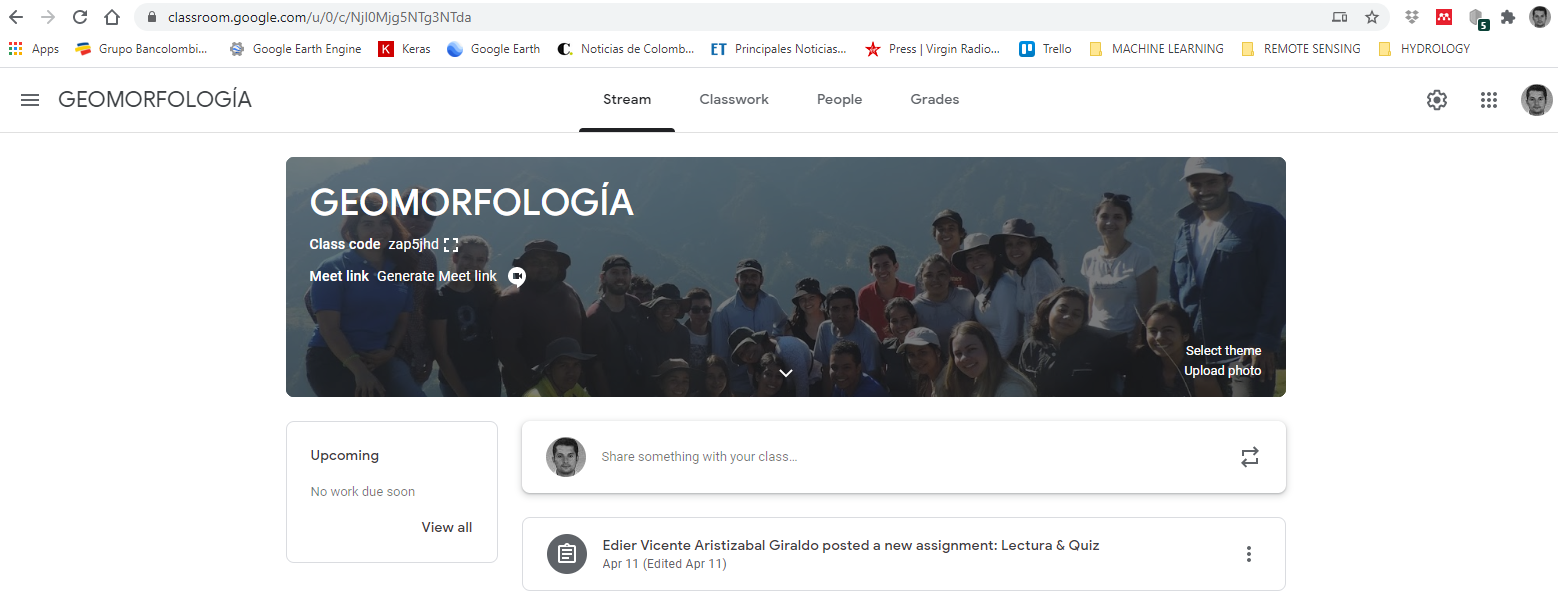
\includegraphics[width=10cm]{classroom}
\end{center}}
\end{frame}
%%%%%%%%%%%%%%%%%%%%%%%%%%%%%%%%%%%%%%%%%%%%%%%%%%%%%%%%%%%%%%%%%
\begin{frame}
\frametitle{Objetivos y alcances del curso}
El curso de geomorfología está orientado para estudiantes de ciencias ambientales que deseen adquirir conocimientos sobre los procesos endógenos y exógenos que modelan las geoformas de la superficie terrestre, y la relación suelo-relieve.\vfill
El alcance de este curso es comprender los procesos de modelación del paisaje con sus geoformas asociadas, y aplicar dichos conocimientos en cartografía.\vfill
Curso teórico ($50$\%) y práctico ($50$\%) de $3$ créditos académicos, lo que significa 9 horas semanales de dedicación en promedio durante todo el semestre... \emph{eso significa unas semanas menos horas y otras muchas mas horas.}
\end{frame}
%%%%%%%%%%%%%%%%%%%%%%%%%%%%%%%%%%%%%%%%%%%%%%%%%%%%%%%%%%%%%%%%%
\begin{frame}
\begin{center}
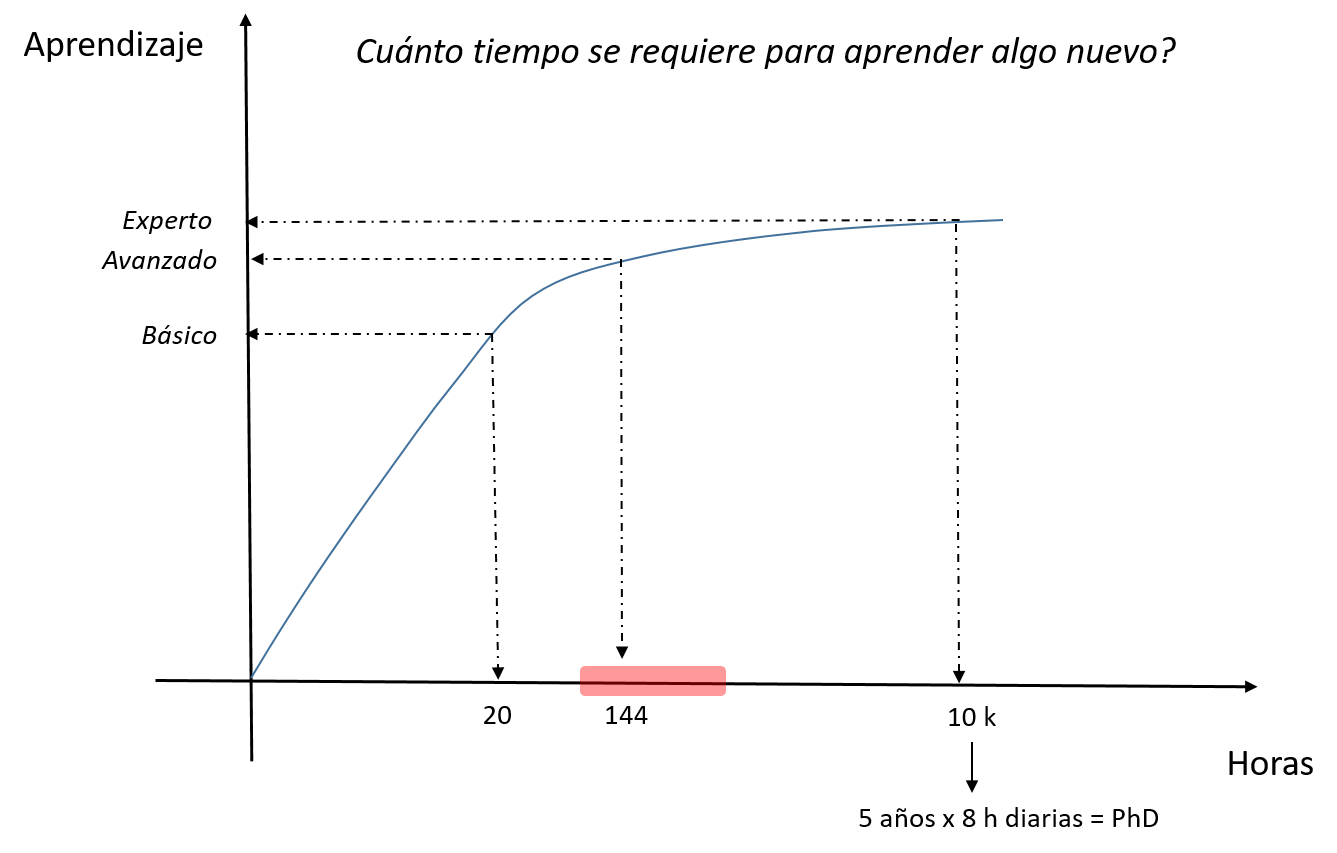
\includegraphics[width=12cm]{curva}
\end{center}
\end{frame}
%%%%%%%%%%%%%%%%%%%%%%%%%%%%%%%%%%%%%%%%%%%%%%%%%%%%%%%%%%%%%%%%%
\begin{frame}
\begin{center}
\includegraphics[width=10cm]{piramide}
\end{center}
\end{frame}
%%%%%%%%%%%%%%%%%%%%%%%%%%%%%%%%%%%%%%%%%%%%%%%%%%%%%%%%%%%%%%%%
\begin{frame}
\begin{center}
\includegraphics[width=12cm]{estrategia}
\end{center}
\end{frame}
%%%%%%%%%%%%%%%%%%%%%%%%%%%%%%%%%%%%%%%%%%%%%%%%%%%%%%%%%%%%%%%%
\begin{frame}
\begin{center}
\includegraphics[width=7cm]{kolb}
\end{center}
\end{frame}
%%%%%%%%%%%%%%%%%%%%%%%%%%%%%%%%%%%%%%%%%%%%%%%%%%%%%%%%%%%%%%%%
%%%
\begin{frame}
\begin{center}
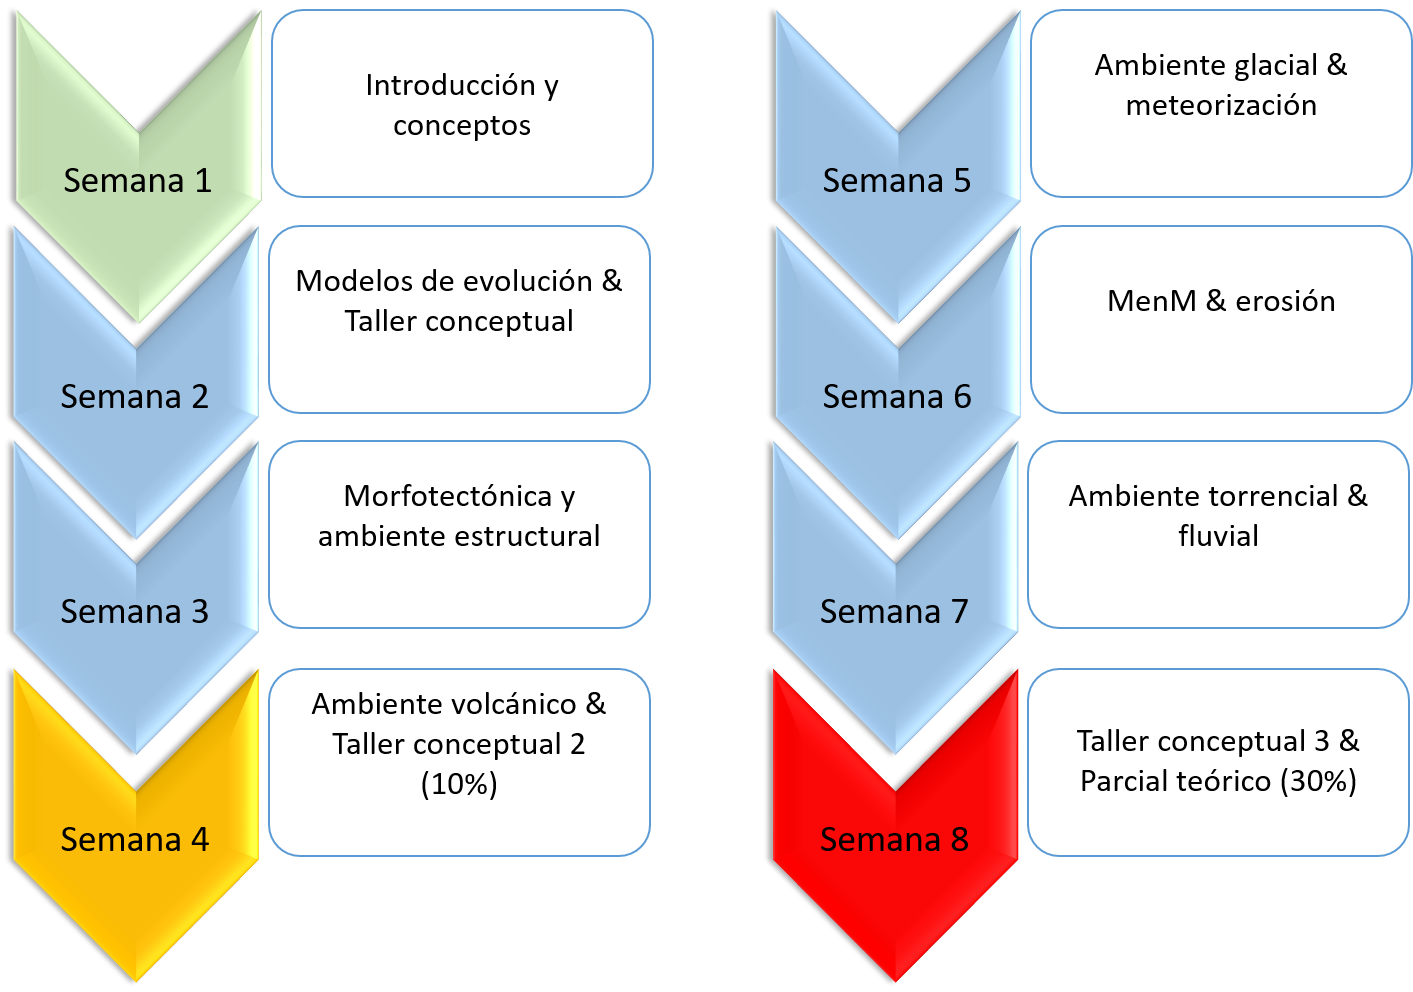
\includegraphics[width=10cm]{crono1}
\end{center}
\end{frame}
%%%%%%%%%%%%%%%%%%%%%%%%%%%%%%%%%%%%%%%%%%%%%%%%%%%%%%%%%%%%%%%%
\begin{frame}
\begin{center}
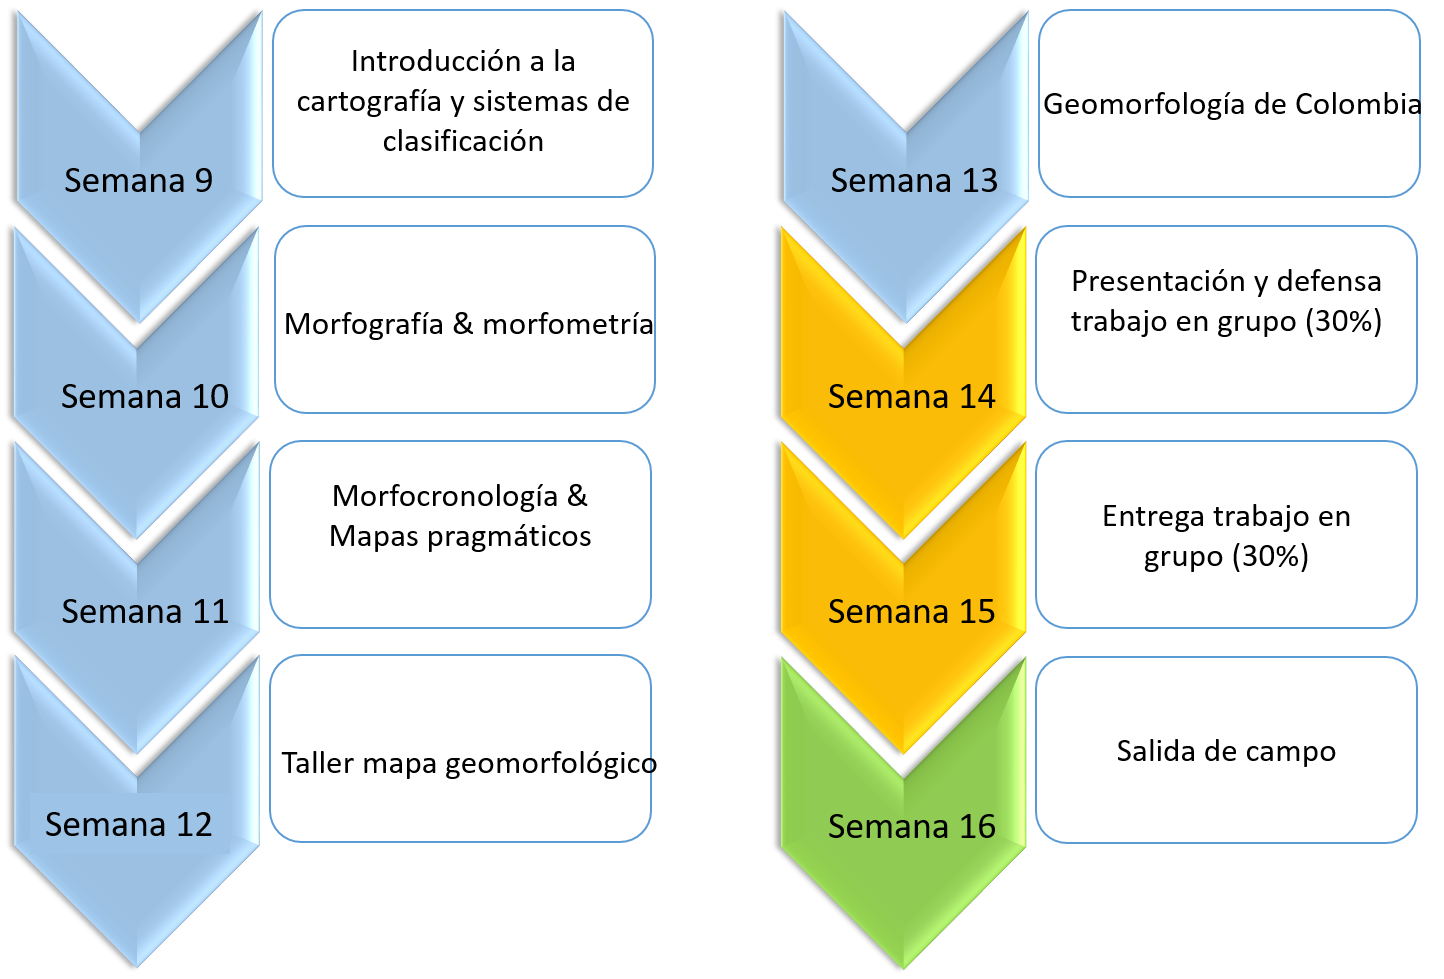
\includegraphics[width=10cm]{crono2}
\end{center}
\end{frame}
%%%%%%%%%%%%%%%%%%%%%%%%%%%%%%%%%%%%%%%%%%%%%%%%%%%%%%%%%%%%%%%%
\begin{frame}
\begin{center}
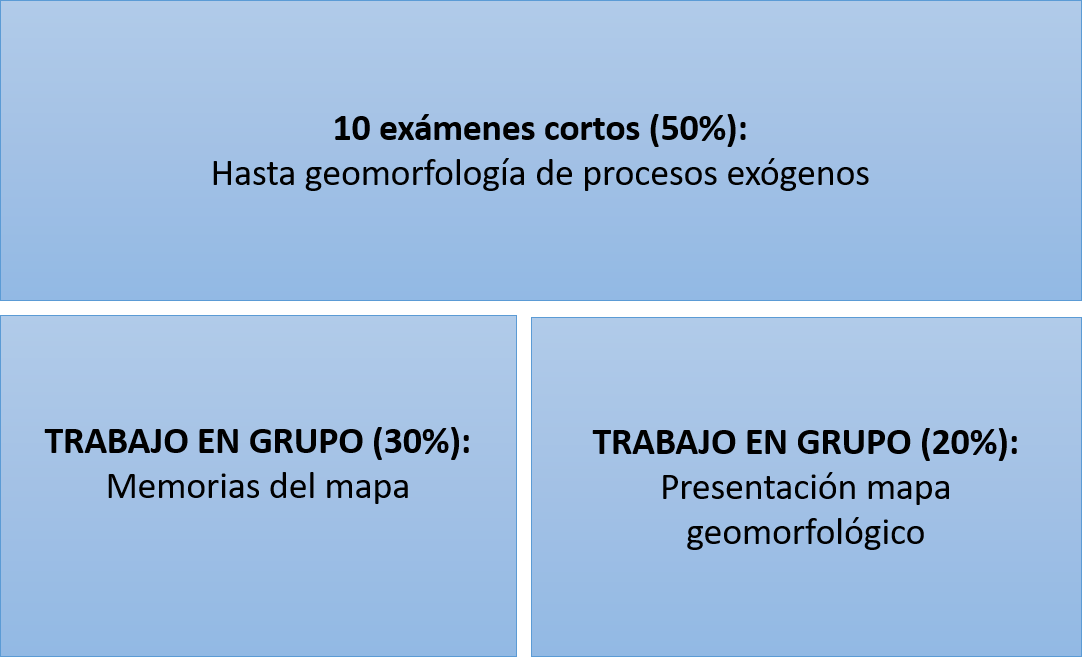
\includegraphics[width=9cm]{cuadro}
\end{center}
\end{frame}
%%%%%%%%%%%%%%%%%%%%%%%%%%%%%%%%%%%%%%%%%%%%%%%%%%%%%%%%%%%%%%%%
\begin{frame}
\begin{center}
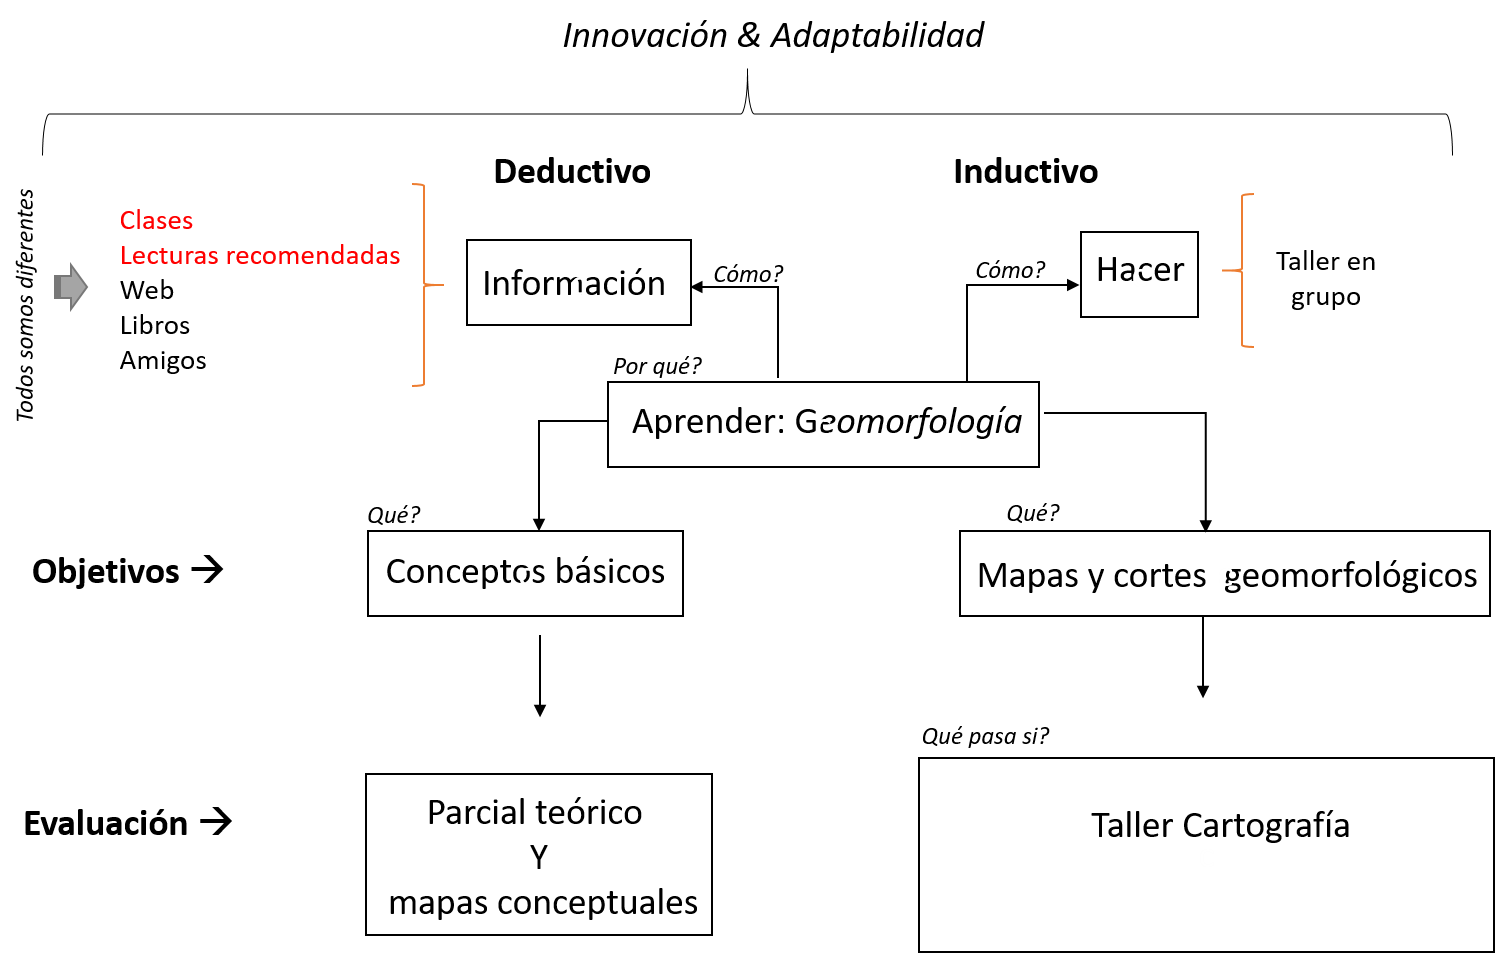
\includegraphics[width=12cm]{abstract}
\end{center}
\end{frame}
%%%%%%%%%%%%%%%%%%%%%%%%%%%%%%%%%%%%%%%%%%%%%%%%%%%%%%%%%%%%%%%%
\end{document}